\section{Results}
\label{sec:results}

% TODO

\begin{table}[H]
\centering
\caption{Overall accuracy (\%) by scaffolding condition and question
category, averaged across all three networks.
Values show mean $\pm$ standard deviation across networks.
Best result per category in \textbf{bold}.}
\label{tab:headline}
\begin{tabular}{lcccc}
\toprule
\textbf{Condition} & \textbf{Retrieval} & \textbf{Reasoning} & \textbf{Multi-step} & \textbf{Overall} \\
\midrule
Naive        & $16.1 \pm 10.2$ & $18.9 \pm 9.2$ & $0.0 \pm 0.0$ & $11.7 \pm 5.4$ \\
SUMO XML     & $88.3 \pm 5.8$ & $27.2 \pm 2.5$ & $10.0 \pm 3.3$ & $41.9 \pm 0.8$ \\
Tool Use     & $\mathbf{100.0 \pm 0.0}$ & $89.4 \pm 1.0$ & $91.1 \pm 5.9$ & $93.5 \pm 1.7$ \\
Plan-Execute-Revise & $\mathbf{100.0 \pm 0.0}$ & $\mathbf{98.9 \pm 1.0}$ & $\mathbf{93.3 \pm 6.0}$ & $\mathbf{97.4 \pm 2.1}$ \\
\bottomrule
\end{tabular}
\end{table}

\FloatBarrier
\begin{table*}[t]
\centering
\caption{Accuracy (\%) of all 36 question types across scaffolding conditions and three SUMO networks.
Best result per row in \textbf{bold}. PER = Plan-Execute-Revise.}
\label{tab:all_results}
\resizebox{0.95\textwidth}{!}{%
\begin{tabular}{l|cccc|cccc|cccc}
\toprule
\multirow{2}{*}{\textbf{Question Type}} & \multicolumn{4}{c|}{\textbf{Grid $8\times8$}} & \multicolumn{4}{c|}{\textbf{Random}} & \multicolumn{4}{c}{\textbf{Times Square}} \\
\cmidrule(lr){2-5} \cmidrule(lr){6-9} \cmidrule(lr){10-13}
 & Naive & XML & Tool Use & PER & Naive & XML & Tool Use & PER & Naive & XML & Tool Use & PER \\
\midrule
\multicolumn{13}{l}{\textbf{Retrieval} (12 types)}\\
Both Junctions              & \textbf{100} & \textbf{100} & \textbf{100} & \textbf{100} & 0 & \textbf{100} & \textbf{100} & \textbf{100} & 0 & \textbf{100} & \textbf{100} & \textbf{100} \\
Num.\ Lanes                 & \textbf{100} & \textbf{100} & \textbf{100} & \textbf{100} & \textbf{100} & \textbf{100} & \textbf{100} & \textbf{100} & 40 & \textbf{100} & \textbf{100} & \textbf{100} \\
Junction Coord.             & 0 & \textbf{100} & \textbf{100} & \textbf{100} & 0 & \textbf{100} & \textbf{100} & \textbf{100} & 0 & \textbf{100} & \textbf{100} & \textbf{100} \\
Veh.\ Depart Time           & 20 & \textbf{100} & \textbf{100} & \textbf{100} & 0 & \textbf{100} & \textbf{100} & \textbf{100} & 0 & \textbf{100} & \textbf{100} & \textbf{100} \\
Veh.\ Depart Edge           & 0 & \textbf{100} & \textbf{100} & \textbf{100} & 0 & \textbf{100} & \textbf{100} & \textbf{100} & 0 & \textbf{100} & \textbf{100} & \textbf{100} \\
Vehicle Route               & 0 & 80 & \textbf{100} & \textbf{100} & 0 & \textbf{100} & \textbf{100} & \textbf{100} & 0 & \textbf{100} & \textbf{100} & \textbf{100} \\
Same-Origin Count           & 0 & 0 & \textbf{100} & \textbf{100} & 0 & \textbf{100} & \textbf{100} & \textbf{100} & 0 & \textbf{100} & \textbf{100} & \textbf{100} \\
Veh.\ Travel Time           & 0 & \textbf{100} & \textbf{100} & \textbf{100} & 0 & \textbf{100} & \textbf{100} & \textbf{100} & 0 & \textbf{100} & \textbf{100} & \textbf{100} \\
Veh.\ Arrival Time          & 0 & \textbf{100} & \textbf{100} & \textbf{100} & 20 & \textbf{100} & \textbf{100} & \textbf{100} & 0 & \textbf{100} & \textbf{100} & \textbf{100} \\
Veh.\ Speed at Time         & 0 & 0 & \textbf{100} & \textbf{100} & 0 & 0 & \textbf{100} & \textbf{100} & 20 & 0 & \textbf{100} & \textbf{100} \\
TLS Phase Count             & 80 & \textbf{100} & \textbf{100} & \textbf{100} & 80 & \textbf{100} & \textbf{100} & \textbf{100} & 0 & \textbf{100} & \textbf{100} & \textbf{100} \\
TLS Longest Green           & 0 & \textbf{100} & \textbf{100} & \textbf{100} & 20 & \textbf{100} & \textbf{100} & \textbf{100} & 0 & \textbf{100} & \textbf{100} & \textbf{100} \\
\cmidrule(lr){1-13}
\textbf{Retrieval Overall}  & 25.0 & 81.7 & \textbf{100.0} & \textbf{100.0} & 18.3 & 91.7 & \textbf{100.0} & \textbf{100.0} & 5.0 & 91.7 & \textbf{100.0} & \textbf{100.0} \\
\midrule
\multicolumn{13}{l}{\textbf{Reasoning} (12 types, single-file)}\\
Shortest Path               & \textbf{100} & \textbf{100} & \textbf{100} & \textbf{100} & 0 & 60 & \textbf{100} & \textbf{100} & 60 & 60 & 80 & \textbf{100} \\
Node Rem.\ Connectivity     & \textbf{100} & 60 & \textbf{100} & \textbf{100} & 20 & 40 & \textbf{100} & \textbf{100} & 60 & \textbf{100} & \textbf{100} & \textbf{100} \\
Bottleneck Edge             & 0 & 20 & 60 & \textbf{100} & 0 & 0 & \textbf{100} & \textbf{100} & 0 & 20 & \textbf{100} & \textbf{100} \\
Avg.\ Route Length          & 20 & 0 & \textbf{100} & \textbf{100} & 0 & \textbf{100} & \textbf{100} & \textbf{100} & 0 & 20 & \textbf{100} & \textbf{100} \\
Route Jaccard Pair          & 0 & 0 & \textbf{80} & \textbf{80} & 0 & 0 & 40 & \textbf{100} & 0 & 0 & 80 & \textbf{100} \\
Route Edit Dist.\ Pair      & 0 & 0 & 60 & \textbf{100} & 0 & 0 & 80 & \textbf{100} & 0 & 0 & 40 & \textbf{100} \\
Route Overlap Count         & 0 & 0 & 80 & \textbf{100} & 0 & 0 & 40 & \textbf{80} & 0 & 0 & 80 & \textbf{100} \\
Highest Timeloss            & 0 & 80 & \textbf{100} & \textbf{100} & 0 & 20 & \textbf{100} & \textbf{100} & 0 & 0 & \textbf{100} & \textbf{100} \\
Avg.\ Trip Duration         & 0 & 0 & \textbf{100} & \textbf{100} & 0 & 0 & \textbf{100} & \textbf{100} & 0 & 0 & \textbf{100} & \textbf{100} \\
Veh.\ Max Speed             & 20 & 0 & \textbf{100} & \textbf{100} & 0 & 0 & \textbf{100} & \textbf{100} & 0 & 0 & \textbf{100} & \textbf{100} \\
Edge Peak Veh.\ Count       & 0 & 0 & \textbf{100} & \textbf{100} & 0 & 0 & \textbf{100} & \textbf{100} & 0 & 0 & \textbf{100} & \textbf{100} \\
TLS Cycle Time              & \textbf{100} & \textbf{100} & \textbf{100} & \textbf{100} & \textbf{100} & \textbf{100} & \textbf{100} & \textbf{100} & \textbf{100} & \textbf{100} & \textbf{100} & \textbf{100} \\
\cmidrule(lr){1-13}
\textbf{Reasoning Overall}  & 28.3 & 30.0 & 90.0 & \textbf{98.3} & 10.0 & 26.7 & 88.3 & \textbf{98.3} & 18.3 & 25.0 & 90.0 & \textbf{100.0} \\
\midrule
\multicolumn{13}{l}{\textbf{Multi-step reasoning} (12 types, multiple files)}\\
Veh.\ Route Distance        & 0 & \textbf{100} & \textbf{100} & \textbf{100} & 0 & \textbf{100} & \textbf{100} & \textbf{100} & 0 & 60 & \textbf{100} & \textbf{100} \\
Worst Congestion OD         & 0 & 0 & \textbf{100} & \textbf{100} & 0 & 0 & \textbf{100} & \textbf{100} & 0 & 0 & \textbf{100} & \textbf{100} \\
Gap Violations              & 0 & 0 & \textbf{100} & \textbf{100} & 0 & 0 & \textbf{100} & \textbf{100} & 0 & 0 & \textbf{100} & \textbf{100} \\
TLS Delay                   & 0 & 0 & \textbf{100} & \textbf{100} & 0 & 0 & \textbf{100} & \textbf{100} & 0 & 0 & \textbf{100} & \textbf{100} \\
Peak/Off-peak Degrad.       & 0 & 0 & \textbf{80} & \textbf{80} & 0 & 0 & \textbf{100} & \textbf{100} & 0 & 20 & \textbf{80} & \textbf{80} \\
Lane Utilisation            & 0 & 0 & 40 & \textbf{60} & 0 & 0 & \textbf{80} & \textbf{80} & 0 & 0 & 40 & \textbf{80} \\
Incomplete OD               & 0 & 60 & \textbf{100} & 80 & 0 & 20 & \textbf{100} & \textbf{100} & 0 & 0 & \textbf{100} & 80 \\
Junction Blocked            & 0 & 0 & \textbf{100} & \textbf{100} & 0 & 0 & \textbf{100} & \textbf{100} & 0 & 0 & \textbf{100} & \textbf{100} \\
Junction Inflow CV          & 0 & 0 & \textbf{20} & \textbf{20} & 0 & 0 & 80 & \textbf{100} & 0 & 0 & \textbf{100} & \textbf{100} \\
Edge Lane Entropy           & 0 & 0 & 80 & \textbf{100} & 0 & 0 & \textbf{100} & \textbf{100} & 0 & 0 & 80 & \textbf{100} \\
TLS Approach Queue          & 0 & 0 & \textbf{100} & \textbf{100} & 0 & 0 & \textbf{100} & \textbf{100} & 0 & 0 & \textbf{100} & \textbf{100} \\
TLS Vehicle Delay           & 0 & 0 & \textbf{100} & \textbf{100} & 0 & 0 & \textbf{100} & \textbf{100} & 0 & 0 & \textbf{100} & \textbf{100} \\
\cmidrule(lr){1-13}
\textbf{Multi-step Overall} & 0.0 & 13.3 & 85.0 & \textbf{86.7} & 0.0 & 10.0 & 96.7 & \textbf{98.3} & 0.0 & 6.7 & 91.7 & \textbf{95.0} \\
\bottomrule
\end{tabular}%
}
\end{table*}

\FloatBarrier
\begin{table*}[t]
\centering
\caption{Category-level accuracy (\%) across scaffolding conditions and three SUMO networks.
Values show mean $\pm$ standard deviation across the 12 question types within each category.
Best result per column in \textbf{bold}.}
\label{tab:category_summary}
\resizebox{0.95\textwidth}{!}{%
\begin{tabular}{l|ccc|ccc|ccc}
\toprule
\multirow{2}{*}{\textbf{Condition}} & \multicolumn{3}{c|}{\textbf{Grid $8\times8$}} & \multicolumn{3}{c|}{\textbf{Random}} & \multicolumn{3}{c}{\textbf{Times Square}} \\
\cmidrule(lr){2-4} \cmidrule(lr){5-7} \cmidrule(lr){8-10}
 & Ret. & Reas. & Multi. & Ret. & Reas. & Multi. & Ret. & Reas. & Multi. \\
\midrule
Naive               & $25.0 \pm 41.9$ & $28.3 \pm 43.9$ & $0.0 \pm 0.0$ & $18.3 \pm 34.6$ & $10.0 \pm 28.9$ & $0.0 \pm 0.0$ & $5.0 \pm 12.4$ & $18.3 \pm 34.6$ & $0.0 \pm 0.0$ \\
SUMO XML            & $81.7 \pm 38.6$ & $30.0 \pm 42.2$ & $13.3 \pm 32.3$ & $91.7 \pm 28.9$ & $26.7 \pm 39.4$ & $10.0 \pm 28.9$ & $91.7 \pm 28.9$ & $25.0 \pm 39.2$ & $6.7 \pm 17.8$ \\
Tool Use            & $\mathbf{100.0 \pm 0.0}$ & $90.0 \pm 16.0$ & $85.0 \pm 27.1$ & $\mathbf{100.0 \pm 0.0}$ & $88.3 \pm 23.3$ & $96.7 \pm 7.8$ & $\mathbf{100.0 \pm 0.0}$ & $90.0 \pm 18.1$ & $91.7 \pm 18.0$ \\
Plan-Execute-Revise & $\mathbf{100.0 \pm 0.0}$ & $\mathbf{98.3 \pm 5.8}$ & $\mathbf{86.7 \pm 24.6}$ & $\mathbf{100.0 \pm 0.0}$ & $\mathbf{98.3 \pm 5.8}$ & $\mathbf{98.3 \pm 5.8}$ & $\mathbf{100.0 \pm 0.0}$ & $\mathbf{100.0 \pm 0.0}$ & $\mathbf{95.0 \pm 9.0}$ \\
\bottomrule
\end{tabular}%
}
\end{table*}

\FloatBarrier
\begin{table*}[t]
\centering
\caption{Category-level and overall accuracy (\%) across scaffolding conditions and three SUMO networks.
Values show mean $\pm$ standard deviation aggregated over all individual questions within each category.
Best result per row in \textbf{bold}.}
\label{tab:category_overall}
\resizebox{0.95\textwidth}{!}{%
\begin{tabular}{l|cccc|cccc|cccc}
\toprule
\multirow{2}{*}{\textbf{Category}} & \multicolumn{4}{c|}{\textbf{Random}} & \multicolumn{4}{c|}{\textbf{Grid $8\times8$}} & \multicolumn{4}{c}{\textbf{Times Square}} \\
\cmidrule(lr){2-5} \cmidrule(lr){6-9} \cmidrule(lr){10-13}
  & File & XML & ReAct & PER & File & XML & ReAct & PER & File & XML & ReAct & PER \\
\midrule
Retrieval & $18.3 \pm 38.7$ & $91.7 \pm 27.6$ & $\mathbf{100.0 \pm 0.0}$ & $\mathbf{100.0 \pm 0.0}$ & $25.0 \pm 43.3$ & $81.7 \pm 38.7$ & $\mathbf{100.0 \pm 0.0}$ & $\mathbf{100.0 \pm 0.0}$ & $13.3 \pm 34.0$ & $78.3 \pm 41.2$ & $\mathbf{100.0 \pm 0.0}$ & $\mathbf{100.0 \pm 0.0}$ \\
Reasoning & $0.0 \pm 0.0$ & $18.0 \pm 38.4$ & $84.0 \pm 36.7$ & $\mathbf{100.0 \pm 0.0}$ & $14.0 \pm 34.7$ & $20.0 \pm 40.0$ & $84.0 \pm 36.7$ & $\mathbf{94.0 \pm 23.7}$ & $8.0 \pm 27.1$ & $18.0 \pm 38.4$ & $78.0 \pm 41.4$ & $\mathbf{96.0 \pm 19.6}$ \\
\midrule
Multi-step Reasoning & $0.0 \pm 0.0$ & $2.0 \pm 14.0$ & $68.0 \pm 46.6$ & $\mathbf{92.0 \pm 27.1}$ & $0.0 \pm 0.0$ & $6.0 \pm 23.7$ & $60.0 \pm 49.0$ & $\mathbf{84.0 \pm 36.7}$ & $0.0 \pm 0.0$ & $4.0 \pm 19.6$ & $56.0 \pm 49.6$ & $\mathbf{82.0 \pm 38.4}$ \\
\bottomrule
\end{tabular}%
}
\end{table*}

\FloatBarrier

\subsection{Ablation Studies}
\label{sec:ablations}

\begin{table}[t]
\centering
\caption{API ablation: Plan-Execute-Revise (PER) accuracy (\%) by question category for backbone LLMs, pooled across the three SUMO networks. Best per column in \textbf{bold}.}
\label{tab:ablation_api}
\resizebox{\columnwidth}{!}{%
\begin{tabular}{l|ccc}
\toprule
\textbf{Model} & \textbf{Retrieval} & \textbf{Reasoning} & \textbf{Multi-step} \\
\midrule
Claude-Sonnet 4.6 & \textbf{100.0} & \textbf{96.7} & \textbf{86.7} \\
Claude-Haiku 4.5 & \textbf{100.0} & 88.0 & 68.0 \\
GPT-5.4-mini & 95.6 & 96.0 & 72.0 \\
Gemini-3.5-flash & \textbf{100.0} & 68.7 & 48.0 \\
\bottomrule
\end{tabular}%
}
\end{table}


\paragraph{API ablation.}
By default, we instantiate the Plan-Execute-Revise (PER) agent with Claude-Sonnet-4.6. In this section, we further analyze how the choice of backbone LLM affects performance by swapping in three relatively weaker models (Claude-Haiku-4.5, GPT-5.4-mini, and Gemini-3.5-flash). As shown in \Cref{tab:ablation_api}, these weaker models remain competitive on retrieval and reasoning tasks but suffer from performance degradation on multi-step reasoning tasks. It underscores that a strong underlying reasoning capability is crucial precisely for the multi-step tasks that require composing several intermediate steps.

\FloatBarrier
\definecolor{royalblue}{RGB}{65,105,225}
\definecolor{firebrick}{RGB}{178,34,34}
\definecolor{darkgreen}{RGB}{0,100,0}
\begin{figure}[t]
\centering
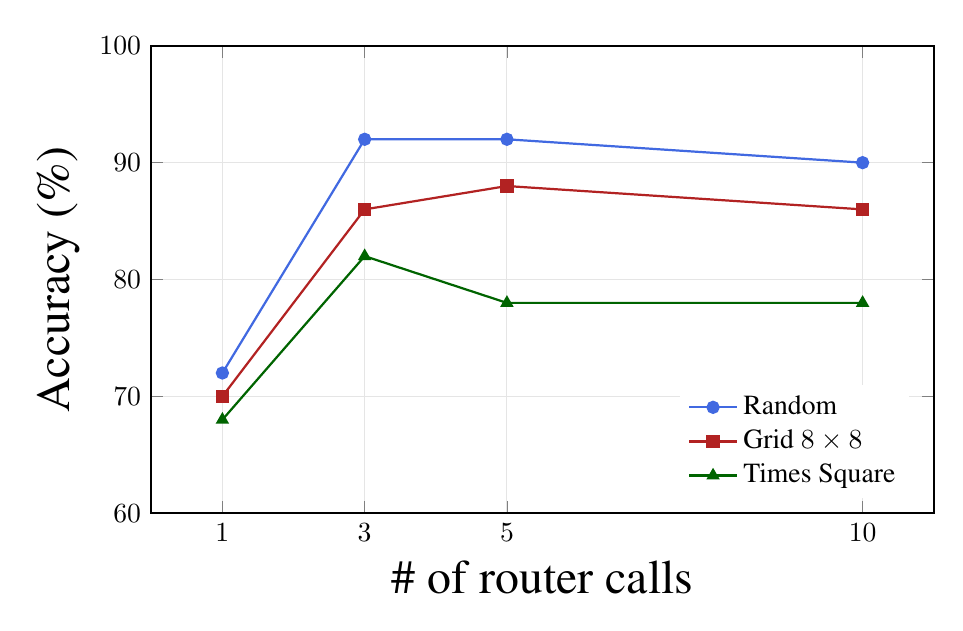
\begin{tikzpicture}[font=\fontfamily{ptm}\selectfont]
\begin{axis}[
    width=0.95\columnwidth, height=0.62\columnwidth,
    xlabel={\# of router calls}, ylabel={Accuracy (\%)},
    label style={font=\LARGE\fontfamily{ptm}\selectfont},
    tick label style={font=\fontfamily{ptm}\selectfont},
    legend style={draw=none, font=\fontfamily{ptm}\selectfont},
    xtick={1,3,5,10},
    xmin=0, xmax=11, ymin=60, ymax=100,
    legend pos=south east, legend cell align={left},
    grid=both, grid style={gray!20}, thick, mark size=2pt,
]
\addplot[royalblue, mark=*] coordinates {(1,72.0) (3,92.0) (5,92.0) (10,90.0)};
\addlegendentry{Random}
\addplot[firebrick, mark=square*] coordinates {(1,70.0) (3,86.0) (5,88.0) (10,86.0)};
\addlegendentry{Grid $8\times8$}
\addplot[darkgreen, mark=triangle*] coordinates {(1,68.0) (3,82.0) (5,78.0) (10,78.0)};
\addlegendentry{Times Square}
\end{axis}
\end{tikzpicture}
\caption{Router-turn ablation: PER accuracy (\%) on the multi-step reasoning tasks as the router-turn budget varies.}
\label{fig:ablation_router_turns}
\end{figure}


\paragraph{Router-turn ablation.}
By default, we set the number of router calls per question at three. Here, we analyze how varying this budget affects performance on the multi-step reasoning tasks. As shown in \Cref{fig:ablation_router_turns}, a single router call is clearly insufficient. Surprisingly, granting additional calls does not improve performance and even slightly degrades it across all three networks. This suggests that three router calls already suffice to gather the evidence required for these tasks, while a larger budget mainly introduces redundant steps that add noise rather than useful information.

\FloatBarrier